\subsubsection{\textit{Whitelisting} pada \textsc{SendGrid}}
	% todo inline numbering
	\textit{Whitelisting} adalah kebalikan dari teknologi \textit{blacklist}. Jika \textit{blacklist} merupakan daftar dari sekumpulan web domain ataupun alamat email, dan URL yang terindikasi tidak “aman” sehingga secara otomatis akan diblokir oleh komputer maupun jaringan agar tidak dapat diakses, maka \textit{whitelist} kebalikan dari \textit{blacklist} yaitu daftar yang diperbolehkan untuk diakses oleh komputer atau jaringan dimana terdapat sekumpulan URL, web domain maupun alamat email yang “aman”.\\
	\indent Masalah dimulai saat \textit{email} konfirmasi akun yang dikirimkan oleh sistem aplikasi lelang online - dengan menggunakan SMTP \textit{relay} - kepada \textit{email pengguna}, masuk ke dalam kotak pesan sebagai \textit{spam}. Hal ini tentu tidak baik - karena seharusnya masuk ke \textit{inbox} sebagaimana \textit{email} pada umumnya. Setelah penulis mencoba mencari jalan keluar, terutama SendGrid tidak menyediakan \textit{whitelisting} dengan menggunakan \textit{root domain} (karena penulis membeli domain lelangapa.com, penulis tidak dapat mengirim \textit{email} konfirmasi akun dengan menggunakan any\_email\_address@lelangapa.com, dan hingga buku ini ditulis penulis tetap tidak tahu alasan pastinya apa). Masalah ini baru selesai dengan menggunakan pemecahan berikut:
	\begin{enumerate}
		\item Membuat sebuah domain noreply.lelangapa.com
		\item Me\textit{register} domain \textit{whitelisting} di pengaturan SendGrid
	\end{enumerate}
	
	\begin{figure}[H]
		\centering
		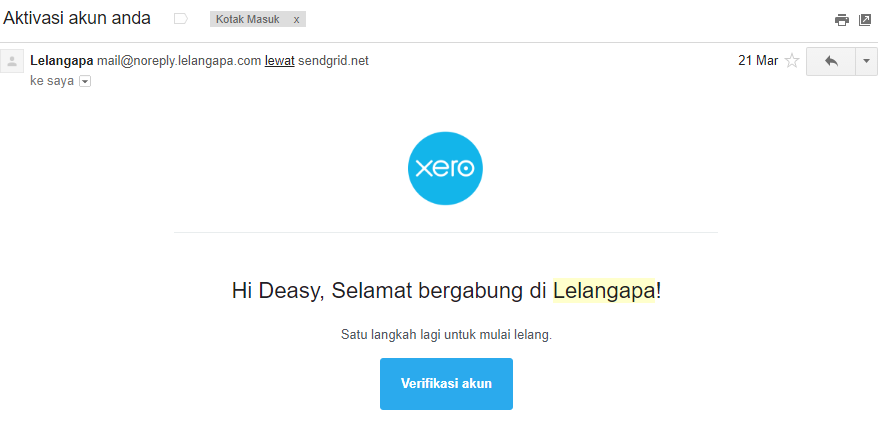
\includegraphics[width=\textwidth]{images/bab4/pl/whitelist-success.png}
		\caption{\textit{Whitelisting}}
		\label{whitelist-success}
	\end{figure}
	
	\indent 
	\begin{figure}[H]
		\centering
		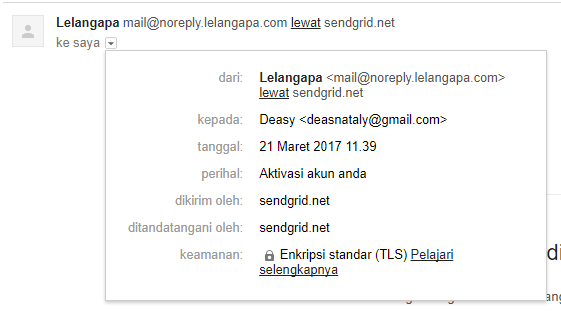
\includegraphics[width=\textwidth]{images/bab4/pl/detail-whitelist.png}
		\caption{Detail Informasi Email yang Masuk ke Kotak Masuk Pengguna}
		\label{detail-whitelist}
	\end{figure}
	